Our test were performed mainly on two machines: one with an Intel® Core i7-7700 @ $3.6 \ GHz$ with $16 \ GB$ of RAM and one on an Amd® Ryzen 7 @ $3.6 \ GHz$ with $32 \ GB$ of RAM.
\subsection{PERM algorithm}
We want now to report an application of the PERM algorithm, made following the article's recipe \cite{PERM}.
The goal of this algorithm is to estimate the total number of fold and then simulate a finite number of SRCs hoping to find the energy minimum.
In the article the number of iterations is set to be $10^5$ for all proteins and the result is that they found only local minima, which are intermediate states.
Our goal is to improve these 2D simulations by increasing the number of iterations, hoping to find the real minimum reported in a famous benchmark \cite{bench}.

The first protein for which we've improved the result is $HH(P)^5HH(P)^3H(P)^3HP$, that has a length of 18 amino acids (see Fig. \ref{fig:18_1}).
In particular, we've found $(1.25 \pm 0.35) \times 10^8$ folds with an energy minimum of -4 (a.u.), equal to the benchmark's one.
\begin{figure}[H]
    \centering
    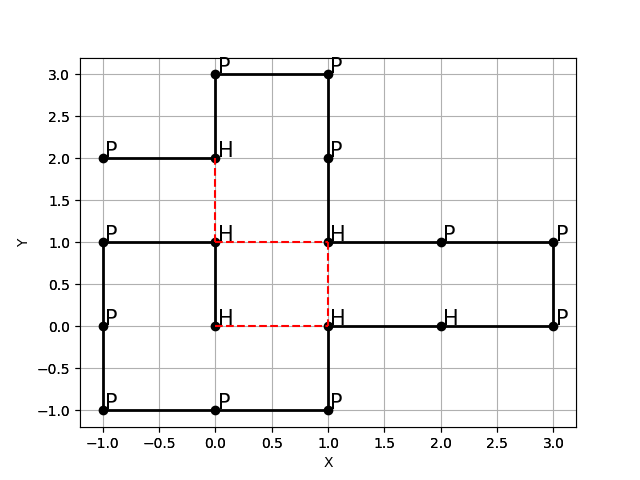
\includegraphics[width=.75\textwidth]{./img/18_1.png}
    \caption{\emph{The protein $HH(P)^5HH(P)^3H(P)^3HP$ has reached its energy minimum at -4 (a.u.) after $5 \times 10^6$ iterations.}}
    \label{fig:18_1}
\end{figure}
Another protein for which we've improved the result is $HHHP(PH)^3PP(HP)^3PH$, that has a length of 20 amino acids (see Fig. \ref{fig:20_2}).
In this case, we've found $(8.9688 \pm 0.0033) \times 10^{10}$ folds with an energy minimum of -9 (a.u.), one unit more than the benchmark's one.
\begin{figure}[H]
    \centering
    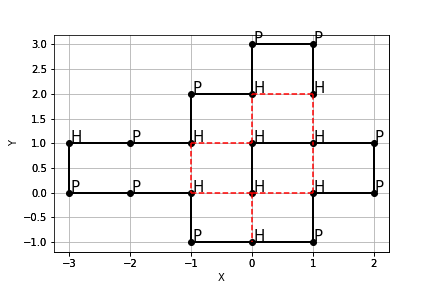
\includegraphics[width=.75\textwidth]{./img/20_2.png}
    \caption{\emph{The protein $HHHP(PH)^3PP(HP)^3PH$ has reached an energy minimum of -9 (a.u.) after $10^7$ iterations.}}
    \label{fig:20_2}
\end{figure}
We've also tried to improve the protein $HPHPHHH(P)^3HHHH(P)^2HH$, that has a length of 20 amino acids (see Fig. \ref{fig:18_2}).
However, after about 5 hours of running time it has folded with an energy of -7 (a.u.), like in the article, with an estimated number of folds equal to $(1.24 \pm 0.43) \times 10^8$.
\begin{figure}[H]
    \centering
    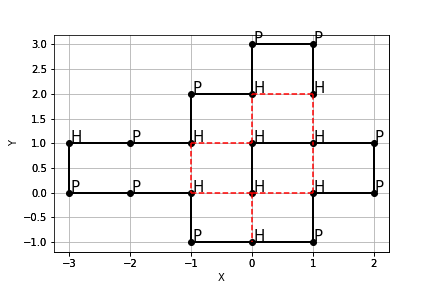
\includegraphics[width=.75\textwidth]{./img/20_2.png}
    \caption{\emph{The protein $HPHPHHH(P)^3HHHH(P)^2HH$ has reached an energy minimum of -7 (a.u.) after $10^8$ iterations.}}
    \label{fig:18_2}
\end{figure}